% Horizontal bar chart: success rate per PROCESS metric across 9 runs
% Usage: % Horizontal bar chart: success rate per PROCESS metric across 9 runs
% Usage: % Horizontal bar chart: success rate per PROCESS metric across 9 runs
% Usage: % Horizontal bar chart: success rate per PROCESS metric across 9 runs
% Usage: \input{generated/variability-process.tex}

\definecolor{cProc}{HTML}{4472C4}

\begin{figure}[H]
\centering
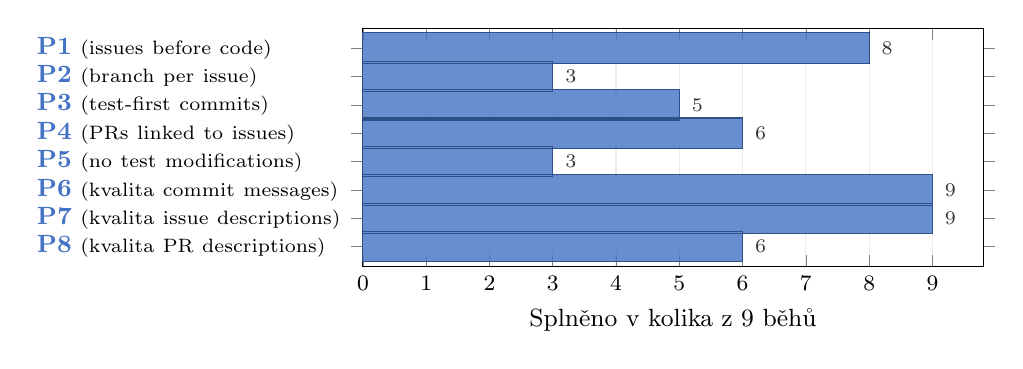
\begin{tikzpicture}
\begin{axis}[
    xbar,
    width=0.78\textwidth,
    height=0.38\textwidth,
    xlabel={Splněno v~kolika z~9 běhů},
    xmin=0, xmax=9.8,
    xtick={0,1,2,3,4,5,6,7,8,9},
    ymin=0.3, ymax=8.7,
    ytick={1,2,3,4,5,6,7,8},
    yticklabels={
        {\textcolor{cProc}{\textbf{P8}} {\scriptsize(kvalita PR descriptions)}},
        {\textcolor{cProc}{\textbf{P7}} {\scriptsize(kvalita issue descriptions)}},
        {\textcolor{cProc}{\textbf{P6}} {\scriptsize(kvalita commit messages)}},
        {\textcolor{cProc}{\textbf{P5}} {\scriptsize(no test modifications)}},
        {\textcolor{cProc}{\textbf{P4}} {\scriptsize(PRs linked to issues)}},
        {\textcolor{cProc}{\textbf{P3}} {\scriptsize(test-first commits)}},
        {\textcolor{cProc}{\textbf{P2}} {\scriptsize(branch per issue)}},
        {\textcolor{cProc}{\textbf{P1}} {\scriptsize(issues before code)}}
    },
    yticklabel style={font=\small, anchor=east, text width=11em, align=left},
    xticklabel style={font=\footnotesize},
    xlabel style={font=\small},
    bar width=11pt,
    nodes near coords,
    nodes near coords style={font=\scriptsize, anchor=west, xshift=1pt},
    xmajorgrids=true,
    ymajorgrids=false,
    grid style={gray!15},
    clip=false,
]

\addplot[fill=cProc, draw=cProc!70!black, fill opacity=0.8] coordinates {
    (6,1)   % P8 >=2/3: 6/9
    (9,2)   % P7 >=2/3: 9/9
    (9,3)   % P6 >=2/3: 9/9
    (3,4)   % P5: 3/9
    (6,5)   % P4: 6/9
    (5,6)   % P3: 5/9
    (3,7)   % P2: 3/9
    (8,8)   % P1: 8/9
};

\end{axis}
\end{tikzpicture}
\caption{Míra splnění exit kritérií \mgrp{P} napříč devíti běhy
(deterministické \acs{P1}--\acs{P5}: pass; judge-based
\acs{P6}--\acs{P8}: $\geq$~2/3).
\acs{P2} a~\acs{P5} byly splněny nejméně často (3/9),
\acs{P6} a~\acs{P7} ve všech bězích.
Deterministické položky (\acs{P1}--\acs{P5}) vykazují vyšší variabilitu
než kvalitativní (\acs{P6}--\acs{P8}).}
\label{fig:variability-process}
\end{figure}


\definecolor{cProc}{HTML}{4472C4}

\begin{figure}[H]
\centering
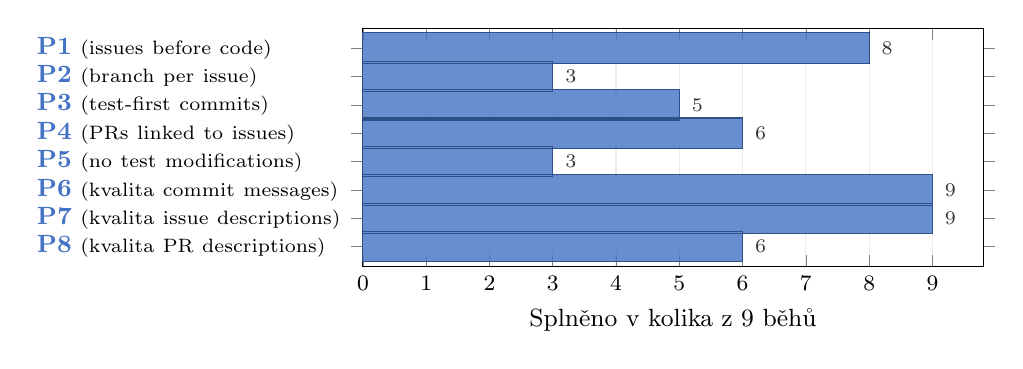
\begin{tikzpicture}
\begin{axis}[
    xbar,
    width=0.78\textwidth,
    height=0.38\textwidth,
    xlabel={Splněno v~kolika z~9 běhů},
    xmin=0, xmax=9.8,
    xtick={0,1,2,3,4,5,6,7,8,9},
    ymin=0.3, ymax=8.7,
    ytick={1,2,3,4,5,6,7,8},
    yticklabels={
        {\textcolor{cProc}{\textbf{P8}} {\scriptsize(kvalita PR descriptions)}},
        {\textcolor{cProc}{\textbf{P7}} {\scriptsize(kvalita issue descriptions)}},
        {\textcolor{cProc}{\textbf{P6}} {\scriptsize(kvalita commit messages)}},
        {\textcolor{cProc}{\textbf{P5}} {\scriptsize(no test modifications)}},
        {\textcolor{cProc}{\textbf{P4}} {\scriptsize(PRs linked to issues)}},
        {\textcolor{cProc}{\textbf{P3}} {\scriptsize(test-first commits)}},
        {\textcolor{cProc}{\textbf{P2}} {\scriptsize(branch per issue)}},
        {\textcolor{cProc}{\textbf{P1}} {\scriptsize(issues before code)}}
    },
    yticklabel style={font=\small, anchor=east, text width=11em, align=left},
    xticklabel style={font=\footnotesize},
    xlabel style={font=\small},
    bar width=11pt,
    nodes near coords,
    nodes near coords style={font=\scriptsize, anchor=west, xshift=1pt},
    xmajorgrids=true,
    ymajorgrids=false,
    grid style={gray!15},
    clip=false,
]

\addplot[fill=cProc, draw=cProc!70!black, fill opacity=0.8] coordinates {
    (6,1)   % P8 >=2/3: 6/9
    (9,2)   % P7 >=2/3: 9/9
    (9,3)   % P6 >=2/3: 9/9
    (3,4)   % P5: 3/9
    (6,5)   % P4: 6/9
    (5,6)   % P3: 5/9
    (3,7)   % P2: 3/9
    (8,8)   % P1: 8/9
};

\end{axis}
\end{tikzpicture}
\caption{Míra splnění exit kritérií \mgrp{P} napříč devíti běhy
(deterministické \acs{P1}--\acs{P5}: pass; judge-based
\acs{P6}--\acs{P8}: $\geq$~2/3).
\acs{P2} a~\acs{P5} byly splněny nejméně často (3/9),
\acs{P6} a~\acs{P7} ve všech bězích.
Deterministické položky (\acs{P1}--\acs{P5}) vykazují vyšší variabilitu
než kvalitativní (\acs{P6}--\acs{P8}).}
\label{fig:variability-process}
\end{figure}


\definecolor{cProc}{HTML}{4472C4}

\begin{figure}[H]
\centering
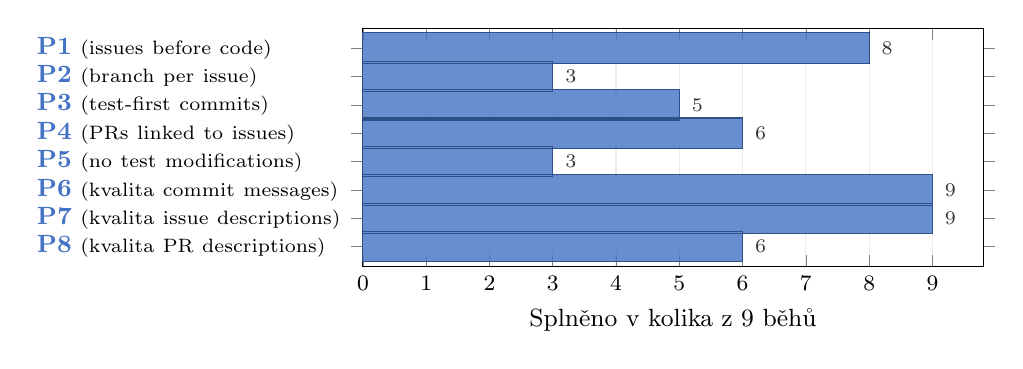
\begin{tikzpicture}
\begin{axis}[
    xbar,
    width=0.78\textwidth,
    height=0.38\textwidth,
    xlabel={Splněno v~kolika z~9 běhů},
    xmin=0, xmax=9.8,
    xtick={0,1,2,3,4,5,6,7,8,9},
    ymin=0.3, ymax=8.7,
    ytick={1,2,3,4,5,6,7,8},
    yticklabels={
        {\textcolor{cProc}{\textbf{P8}} {\scriptsize(kvalita PR descriptions)}},
        {\textcolor{cProc}{\textbf{P7}} {\scriptsize(kvalita issue descriptions)}},
        {\textcolor{cProc}{\textbf{P6}} {\scriptsize(kvalita commit messages)}},
        {\textcolor{cProc}{\textbf{P5}} {\scriptsize(no test modifications)}},
        {\textcolor{cProc}{\textbf{P4}} {\scriptsize(PRs linked to issues)}},
        {\textcolor{cProc}{\textbf{P3}} {\scriptsize(test-first commits)}},
        {\textcolor{cProc}{\textbf{P2}} {\scriptsize(branch per issue)}},
        {\textcolor{cProc}{\textbf{P1}} {\scriptsize(issues before code)}}
    },
    yticklabel style={font=\small, anchor=east, text width=11em, align=left},
    xticklabel style={font=\footnotesize},
    xlabel style={font=\small},
    bar width=11pt,
    nodes near coords,
    nodes near coords style={font=\scriptsize, anchor=west, xshift=1pt},
    xmajorgrids=true,
    ymajorgrids=false,
    grid style={gray!15},
    clip=false,
]

\addplot[fill=cProc, draw=cProc!70!black, fill opacity=0.8] coordinates {
    (6,1)   % P8 >=2/3: 6/9
    (9,2)   % P7 >=2/3: 9/9
    (9,3)   % P6 >=2/3: 9/9
    (3,4)   % P5: 3/9
    (6,5)   % P4: 6/9
    (5,6)   % P3: 5/9
    (3,7)   % P2: 3/9
    (8,8)   % P1: 8/9
};

\end{axis}
\end{tikzpicture}
\caption{Míra splnění exit kritérií \mgrp{P} napříč devíti běhy
(deterministické \acs{P1}--\acs{P5}: pass; judge-based
\acs{P6}--\acs{P8}: $\geq$~2/3).
\acs{P2} a~\acs{P5} byly splněny nejméně často (3/9),
\acs{P6} a~\acs{P7} ve všech bězích.
Deterministické položky (\acs{P1}--\acs{P5}) vykazují vyšší variabilitu
než kvalitativní (\acs{P6}--\acs{P8}).}
\label{fig:variability-process}
\end{figure}


\definecolor{cProc}{HTML}{4472C4}

\begin{figure}[H]
\centering
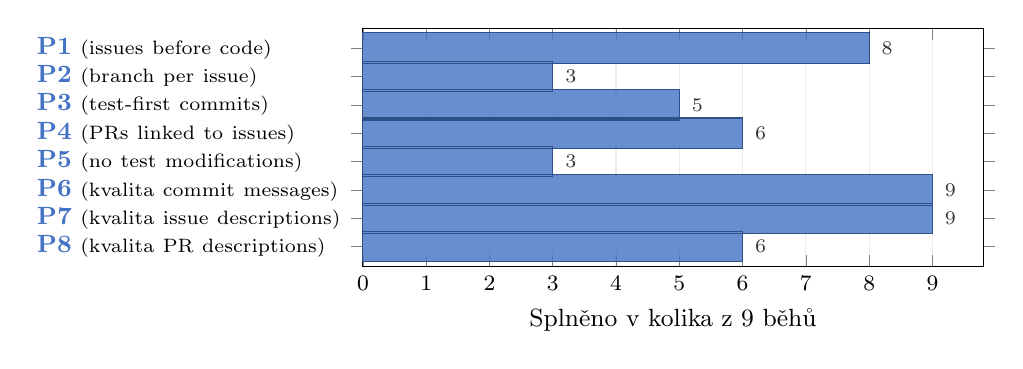
\begin{tikzpicture}
\begin{axis}[
    xbar,
    width=0.78\textwidth,
    height=0.38\textwidth,
    xlabel={Splněno v~kolika z~9 běhů},
    xmin=0, xmax=9.8,
    xtick={0,1,2,3,4,5,6,7,8,9},
    ymin=0.3, ymax=8.7,
    ytick={1,2,3,4,5,6,7,8},
    yticklabels={
        {\textcolor{cProc}{\textbf{P8}} {\scriptsize(kvalita PR descriptions)}},
        {\textcolor{cProc}{\textbf{P7}} {\scriptsize(kvalita issue descriptions)}},
        {\textcolor{cProc}{\textbf{P6}} {\scriptsize(kvalita commit messages)}},
        {\textcolor{cProc}{\textbf{P5}} {\scriptsize(no test modifications)}},
        {\textcolor{cProc}{\textbf{P4}} {\scriptsize(PRs linked to issues)}},
        {\textcolor{cProc}{\textbf{P3}} {\scriptsize(test-first commits)}},
        {\textcolor{cProc}{\textbf{P2}} {\scriptsize(branch per issue)}},
        {\textcolor{cProc}{\textbf{P1}} {\scriptsize(issues before code)}}
    },
    yticklabel style={font=\small, anchor=east, text width=11em, align=left},
    xticklabel style={font=\footnotesize},
    xlabel style={font=\small},
    bar width=11pt,
    nodes near coords,
    nodes near coords style={font=\scriptsize, anchor=west, xshift=1pt},
    xmajorgrids=true,
    ymajorgrids=false,
    grid style={gray!15},
    clip=false,
]

\addplot[fill=cProc, draw=cProc!70!black, fill opacity=0.8] coordinates {
    (6,1)   % P8 >=2/3: 6/9
    (9,2)   % P7 >=2/3: 9/9
    (9,3)   % P6 >=2/3: 9/9
    (3,4)   % P5: 3/9
    (6,5)   % P4: 6/9
    (5,6)   % P3: 5/9
    (3,7)   % P2: 3/9
    (8,8)   % P1: 8/9
};

\end{axis}
\end{tikzpicture}
\caption{Míra splnění exit kritérií \mgrp{P} napříč devíti běhy
(deterministické \acs{P1}--\acs{P5}: pass; judge-based
\acs{P6}--\acs{P8}: $\geq$~2/3).
\acs{P2} a~\acs{P5} byly splněny nejméně často (3/9),
\acs{P6} a~\acs{P7} ve všech bězích.
Deterministické položky (\acs{P1}--\acs{P5}) vykazují vyšší variabilitu
než kvalitativní (\acs{P6}--\acs{P8}).}
\label{fig:variability-process}
\end{figure}
